% Options for packages loaded elsewhere
\PassOptionsToPackage{unicode}{hyperref}
\PassOptionsToPackage{hyphens}{url}
\PassOptionsToPackage{dvipsnames,svgnames,x11names}{xcolor}
%
\documentclass[
  letterpaper,
  DIV=11,
  numbers=noendperiod]{scrreprt}

\usepackage{amsmath,amssymb}
\usepackage{iftex}
\ifPDFTeX
  \usepackage[T1]{fontenc}
  \usepackage[utf8]{inputenc}
  \usepackage{textcomp} % provide euro and other symbols
\else % if luatex or xetex
  \usepackage{unicode-math}
  \defaultfontfeatures{Scale=MatchLowercase}
  \defaultfontfeatures[\rmfamily]{Ligatures=TeX,Scale=1}
\fi
\usepackage{lmodern}
\ifPDFTeX\else  
    % xetex/luatex font selection
\fi
% Use upquote if available, for straight quotes in verbatim environments
\IfFileExists{upquote.sty}{\usepackage{upquote}}{}
\IfFileExists{microtype.sty}{% use microtype if available
  \usepackage[]{microtype}
  \UseMicrotypeSet[protrusion]{basicmath} % disable protrusion for tt fonts
}{}
\makeatletter
\@ifundefined{KOMAClassName}{% if non-KOMA class
  \IfFileExists{parskip.sty}{%
    \usepackage{parskip}
  }{% else
    \setlength{\parindent}{0pt}
    \setlength{\parskip}{6pt plus 2pt minus 1pt}}
}{% if KOMA class
  \KOMAoptions{parskip=half}}
\makeatother
\usepackage{xcolor}
\setlength{\emergencystretch}{3em} % prevent overfull lines
\setcounter{secnumdepth}{-\maxdimen} % remove section numbering
% Make \paragraph and \subparagraph free-standing
\makeatletter
\ifx\paragraph\undefined\else
  \let\oldparagraph\paragraph
  \renewcommand{\paragraph}{
    \@ifstar
      \xxxParagraphStar
      \xxxParagraphNoStar
  }
  \newcommand{\xxxParagraphStar}[1]{\oldparagraph*{#1}\mbox{}}
  \newcommand{\xxxParagraphNoStar}[1]{\oldparagraph{#1}\mbox{}}
\fi
\ifx\subparagraph\undefined\else
  \let\oldsubparagraph\subparagraph
  \renewcommand{\subparagraph}{
    \@ifstar
      \xxxSubParagraphStar
      \xxxSubParagraphNoStar
  }
  \newcommand{\xxxSubParagraphStar}[1]{\oldsubparagraph*{#1}\mbox{}}
  \newcommand{\xxxSubParagraphNoStar}[1]{\oldsubparagraph{#1}\mbox{}}
\fi
\makeatother


\providecommand{\tightlist}{%
  \setlength{\itemsep}{0pt}\setlength{\parskip}{0pt}}\usepackage{longtable,booktabs,array}
\usepackage{calc} % for calculating minipage widths
% Correct order of tables after \paragraph or \subparagraph
\usepackage{etoolbox}
\makeatletter
\patchcmd\longtable{\par}{\if@noskipsec\mbox{}\fi\par}{}{}
\makeatother
% Allow footnotes in longtable head/foot
\IfFileExists{footnotehyper.sty}{\usepackage{footnotehyper}}{\usepackage{footnote}}
\makesavenoteenv{longtable}
\usepackage{graphicx}
\makeatletter
\def\maxwidth{\ifdim\Gin@nat@width>\linewidth\linewidth\else\Gin@nat@width\fi}
\def\maxheight{\ifdim\Gin@nat@height>\textheight\textheight\else\Gin@nat@height\fi}
\makeatother
% Scale images if necessary, so that they will not overflow the page
% margins by default, and it is still possible to overwrite the defaults
% using explicit options in \includegraphics[width, height, ...]{}
\setkeys{Gin}{width=\maxwidth,height=\maxheight,keepaspectratio}
% Set default figure placement to htbp
\makeatletter
\def\fps@figure{htbp}
\makeatother
% definitions for citeproc citations
\NewDocumentCommand\citeproctext{}{}
\NewDocumentCommand\citeproc{mm}{%
  \begingroup\def\citeproctext{#2}\cite{#1}\endgroup}
\makeatletter
 % allow citations to break across lines
 \let\@cite@ofmt\@firstofone
 % avoid brackets around text for \cite:
 \def\@biblabel#1{}
 \def\@cite#1#2{{#1\if@tempswa , #2\fi}}
\makeatother
\newlength{\cslhangindent}
\setlength{\cslhangindent}{1.5em}
\newlength{\csllabelwidth}
\setlength{\csllabelwidth}{3em}
\newenvironment{CSLReferences}[2] % #1 hanging-indent, #2 entry-spacing
 {\begin{list}{}{%
  \setlength{\itemindent}{0pt}
  \setlength{\leftmargin}{0pt}
  \setlength{\parsep}{0pt}
  % turn on hanging indent if param 1 is 1
  \ifodd #1
   \setlength{\leftmargin}{\cslhangindent}
   \setlength{\itemindent}{-1\cslhangindent}
  \fi
  % set entry spacing
  \setlength{\itemsep}{#2\baselineskip}}}
 {\end{list}}
\usepackage{calc}
\newcommand{\CSLBlock}[1]{\hfill\break\parbox[t]{\linewidth}{\strut\ignorespaces#1\strut}}
\newcommand{\CSLLeftMargin}[1]{\parbox[t]{\csllabelwidth}{\strut#1\strut}}
\newcommand{\CSLRightInline}[1]{\parbox[t]{\linewidth - \csllabelwidth}{\strut#1\strut}}
\newcommand{\CSLIndent}[1]{\hspace{\cslhangindent}#1}

\usepackage{booktabs}
\usepackage{longtable}
\usepackage{array}
\usepackage{multirow}
\usepackage{wrapfig}
\usepackage{float}
\usepackage{colortbl}
\usepackage{pdflscape}
\usepackage{tabu}
\usepackage{threeparttable}
\usepackage{threeparttablex}
\usepackage[normalem]{ulem}
\usepackage{makecell}
\usepackage{xcolor}
\usepackage{fontspec}
\usepackage{multicol}
\usepackage{hhline}
\newlength\Oldarrayrulewidth
\newlength\Oldtabcolsep
\usepackage{hyperref}
\KOMAoption{captions}{tableheading}
\counterwithout{figure}{chapter}
\makeatletter
\@ifpackageloaded{caption}{}{\usepackage{caption}}
\AtBeginDocument{%
\ifdefined\contentsname
  \renewcommand*\contentsname{Table of contents}
\else
  \newcommand\contentsname{Table of contents}
\fi
\ifdefined\listfigurename
  \renewcommand*\listfigurename{List of Figures}
\else
  \newcommand\listfigurename{List of Figures}
\fi
\ifdefined\listtablename
  \renewcommand*\listtablename{List of Tables}
\else
  \newcommand\listtablename{List of Tables}
\fi
\ifdefined\figurename
  \renewcommand*\figurename{Figure}
\else
  \newcommand\figurename{Figure}
\fi
\ifdefined\tablename
  \renewcommand*\tablename{Table}
\else
  \newcommand\tablename{Table}
\fi
}
\@ifpackageloaded{float}{}{\usepackage{float}}
\floatstyle{ruled}
\@ifundefined{c@chapter}{\newfloat{codelisting}{h}{lop}}{\newfloat{codelisting}{h}{lop}[chapter]}
\floatname{codelisting}{Listing}
\newcommand*\listoflistings{\listof{codelisting}{List of Listings}}
\makeatother
\makeatletter
\makeatother
\makeatletter
\@ifpackageloaded{caption}{}{\usepackage{caption}}
\@ifpackageloaded{subcaption}{}{\usepackage{subcaption}}
\makeatother

\ifLuaTeX
  \usepackage{selnolig}  % disable illegal ligatures
\fi
\usepackage{bookmark}

\IfFileExists{xurl.sty}{\usepackage{xurl}}{} % add URL line breaks if available
\urlstyle{same} % disable monospaced font for URLs
\hypersetup{
  pdftitle={Eastern Bering Sea walleye pollock stock assessment},
  pdfauthor={Jim Ianelli and Carey McGilliard},
  colorlinks=true,
  linkcolor={blue},
  filecolor={Maroon},
  citecolor={Blue},
  urlcolor={Blue},
  pdfcreator={LaTeX via pandoc}}


\title{Eastern Bering Sea walleye pollock stock assessment}
\usepackage{etoolbox}
\makeatletter
\providecommand{\subtitle}[1]{% add subtitle to \maketitle
  \apptocmd{\@title}{\par {\large #1 \par}}{}{}
}
\makeatother
\subtitle{May 2025, CIE review}
\author{Jim Ianelli and Carey McGilliard}
\date{2025-04-01 00:00}

\begin{document}
\maketitle


\begin{verbatim}
NULL
\end{verbatim}

\chapter{Executive Summary}\label{executive-summary}

The work presented below was based on the same data sets used in the
2024 assessment. The first task was to update the model runs to include
the 2023 data. The model runs were updated and the results are presented
below. The model runs were then used to compare the FT-NIR data with the
traditional data sources (BTS and ATS). The results of these comparisons
are presented below. The model fits to the data are presented in the
tables at the end of the document.

\chapter{Comparing FT-NIR compositions with traditional microscope age
estimations}\label{comparing-ft-nir-compositions-with-traditional-microscope-age-estimations}

The fish age and growth lab at the AFSC have endeavored to expand on new
technologies (Helser et al. (2019)).

Examining the abundance-at-age (for design-based estimates of the
bottom-trawl age compositions) we show that in general, the TMA
estimates show a high level of consistency by cohort
(Figure~\ref{fig-consisTMA}). For these same data, when applied to the
FTNIRs age-estimation method, the consistency was lower
(Figure~\ref{fig-consisFTN}).

When preparing the data for the assessment, we plotted out the
proportions-at-age for the TMA data and noted the differences in the
estimates using the FTNIRs age estimates
(Figure~\ref{fig-proportionsFSH}, Figure~\ref{fig-proportionsBTS}, and
Figure~\ref{fig-proportionsATS}). Other preparations involved estimating
the age-determination errors for each method following that of Punt et
al. (2008). For the FTNIRs data, we optionally estimated separate
age-estimation error matrices by gear type. The appearance of the
fleet-aggregated and fleet-specific input data files is shown in
Figure~\ref{fig-dataFile}.

\begin{figure}

\centering{

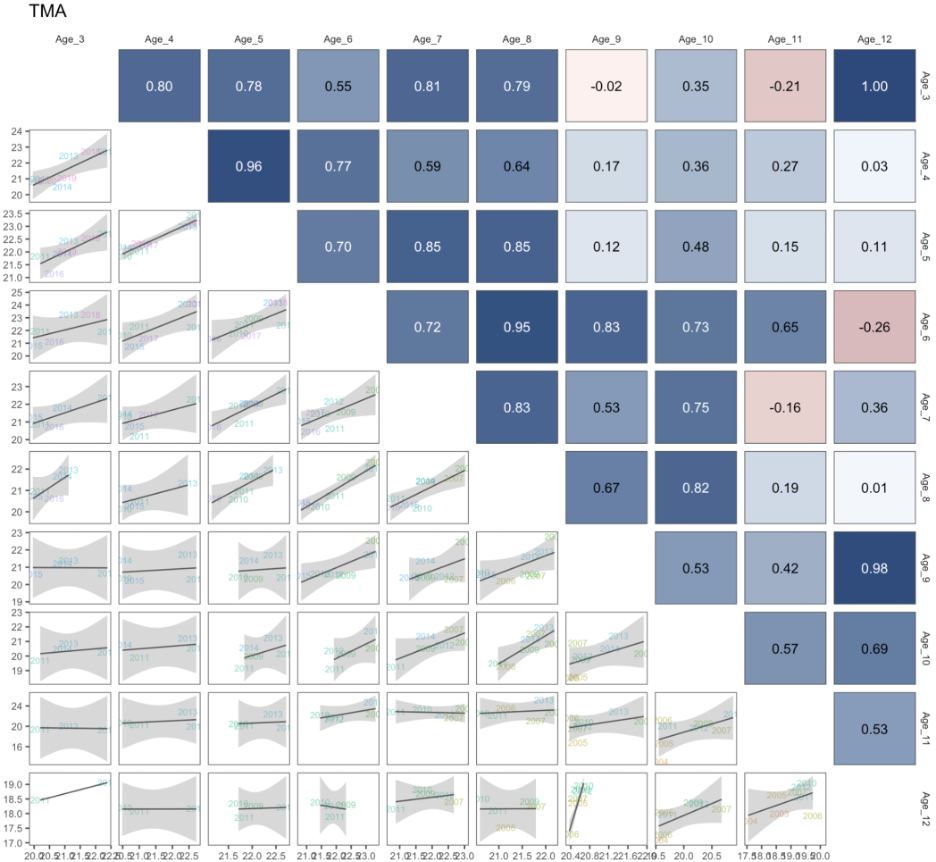
\includegraphics{doc/figs/consisTMA.png}

}

\caption{\label{fig-consisTMA}Cohort consistency over different ages
based on log-abundance from the bottom-trawl survey data for pollock in
recent years for traditional microscope age estimates. The cohorts are
shown in the labels.}

\end{figure}%

\begin{figure}

\centering{

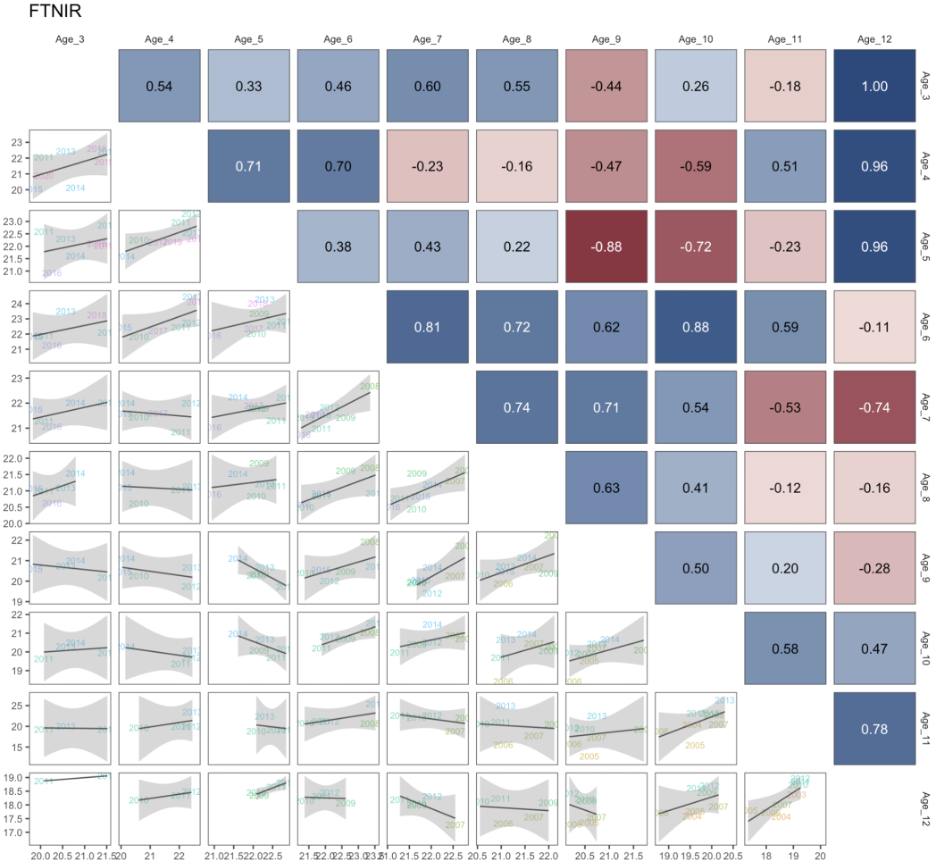
\includegraphics{doc/figs/consisFTN.png}

}

\caption{\label{fig-consisFTN}Cohort consistency over different ages
based on log-abundance from the bottom-trawl survey data for pollock in
recent years for FTNIRs age estimates. The cohorts are shown in the
labels.}

\end{figure}%

\begin{figure}

\centering{

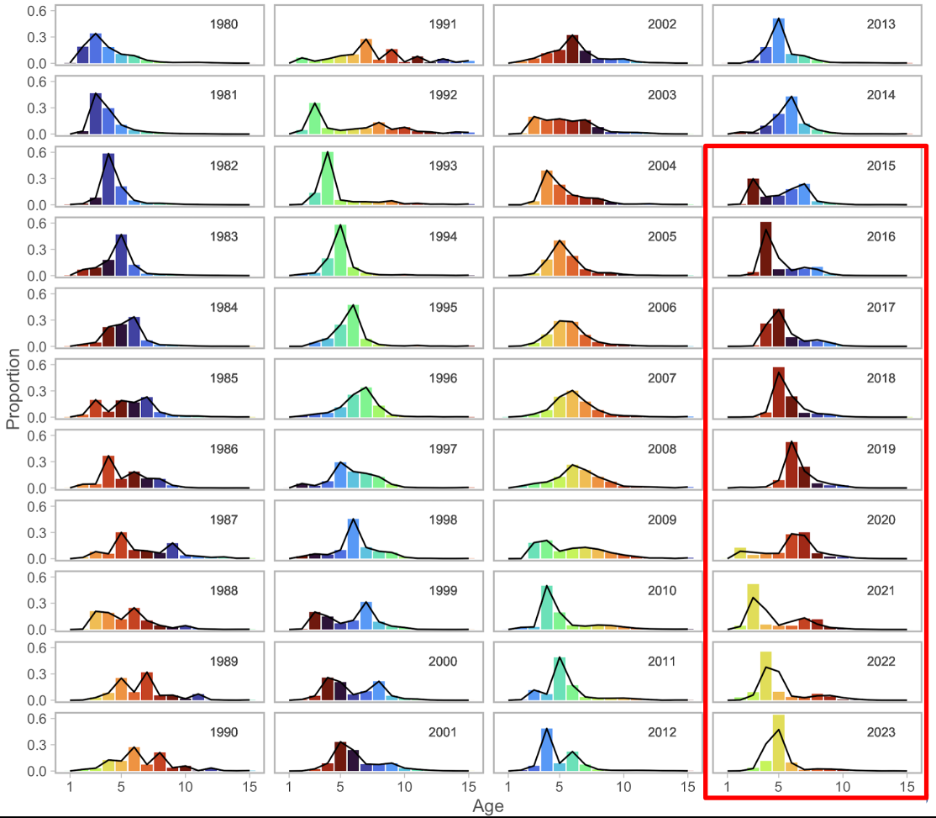
\includegraphics{doc/figs/proportionsFSH.png}

}

\caption{\label{fig-proportionsFSH}Proportions at age for recent years
for the fishery data where the columns represent the traditional
microscope age estimates (TMA) compared to the FTNIRs age estimates
(lines for the red-outlined panels).}

\end{figure}%

\begin{figure}

\centering{

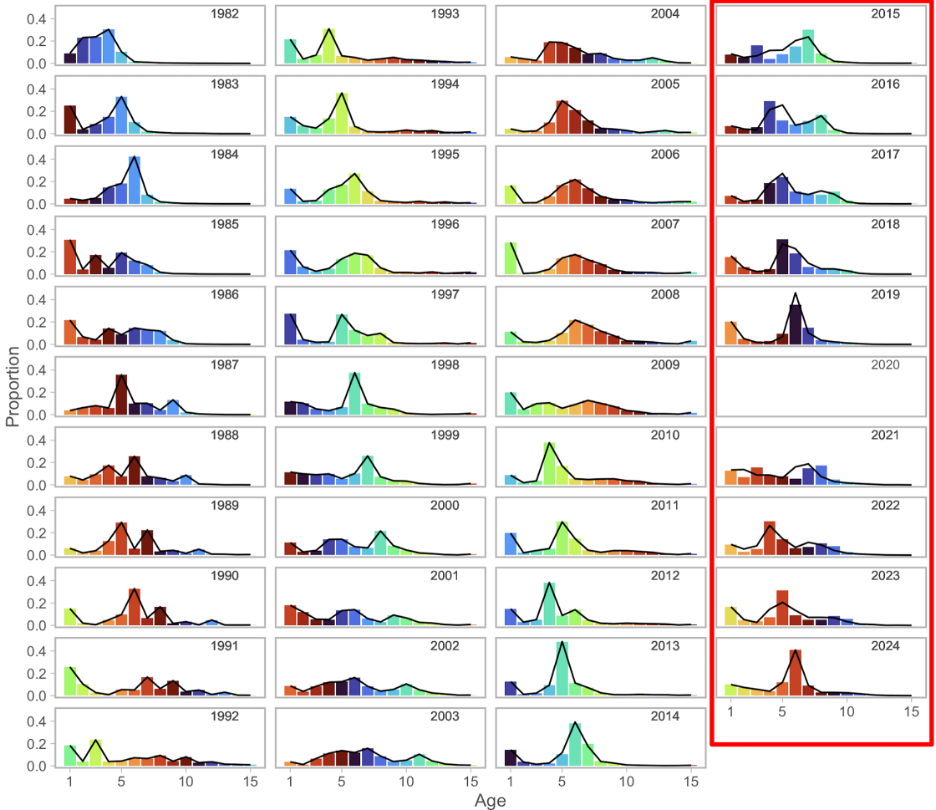
\includegraphics{doc/figs/proportionsBTS.png}

}

\caption{\label{fig-proportionsBTS}Proportions at age for recent years
for the bottom-trawl survey data where the columns represent the
traditional microscope age estimates (TMA) compared to the FTNIRs age
estimates (lines for the red-outlined panels).}

\end{figure}%

\begin{figure}

\centering{

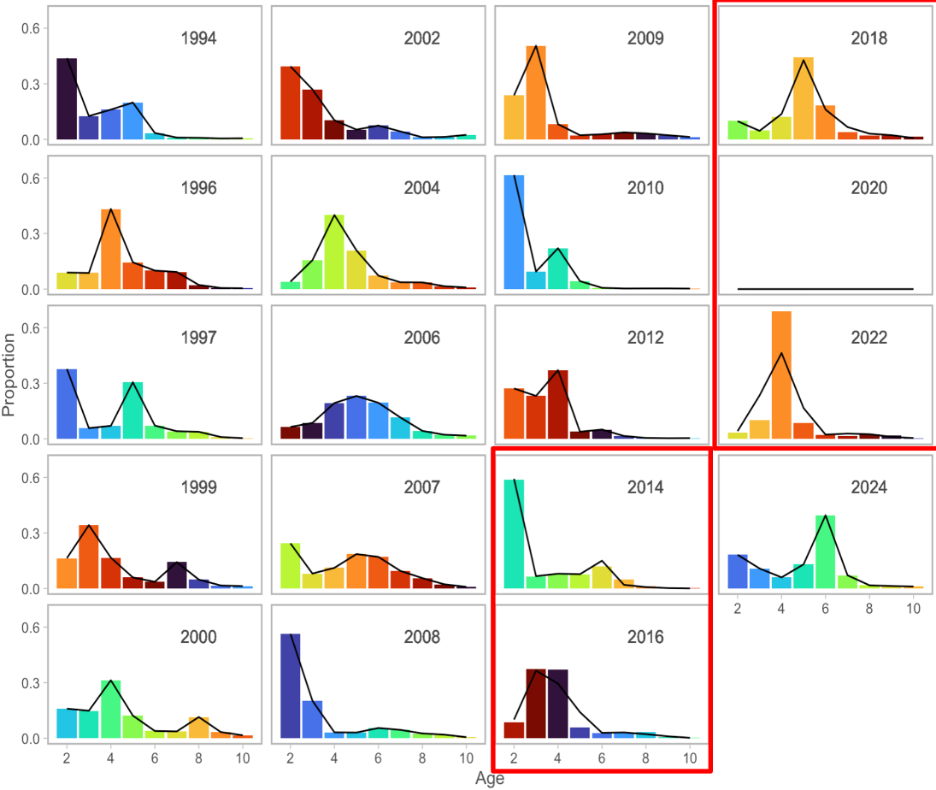
\includegraphics{doc/figs/proportionsATS.png}

}

\caption{\label{fig-proportionsATS}Proportions at age for recent years
for the acoustic-trawl survey data where the columns represent the
traditional microscope age estimates (TMA) compared to the FTNIRs age
estimates (lines for the red-outlined panels).}

\end{figure}%

\begin{figure}

\centering{

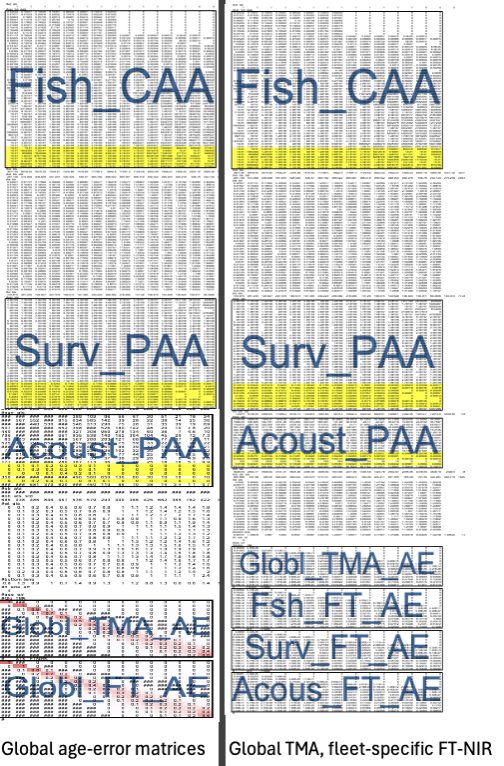
\includegraphics{doc/figs/dataFile.png}

}

\caption{\label{fig-dataFile}Schematic of input datafile showing the
breakout of the fleet-specific FTNIRs age-error matrices (right panel)
compared to that where the global FTNIRs age-error matrices are used
(left panel).}

\end{figure}%

For the assessment model, the alternatives are shown based on the
coverage of data and availability among types of ageing is shown in
Figure~\ref{fig-dataExtent}.

\begin{figure}

\centering{

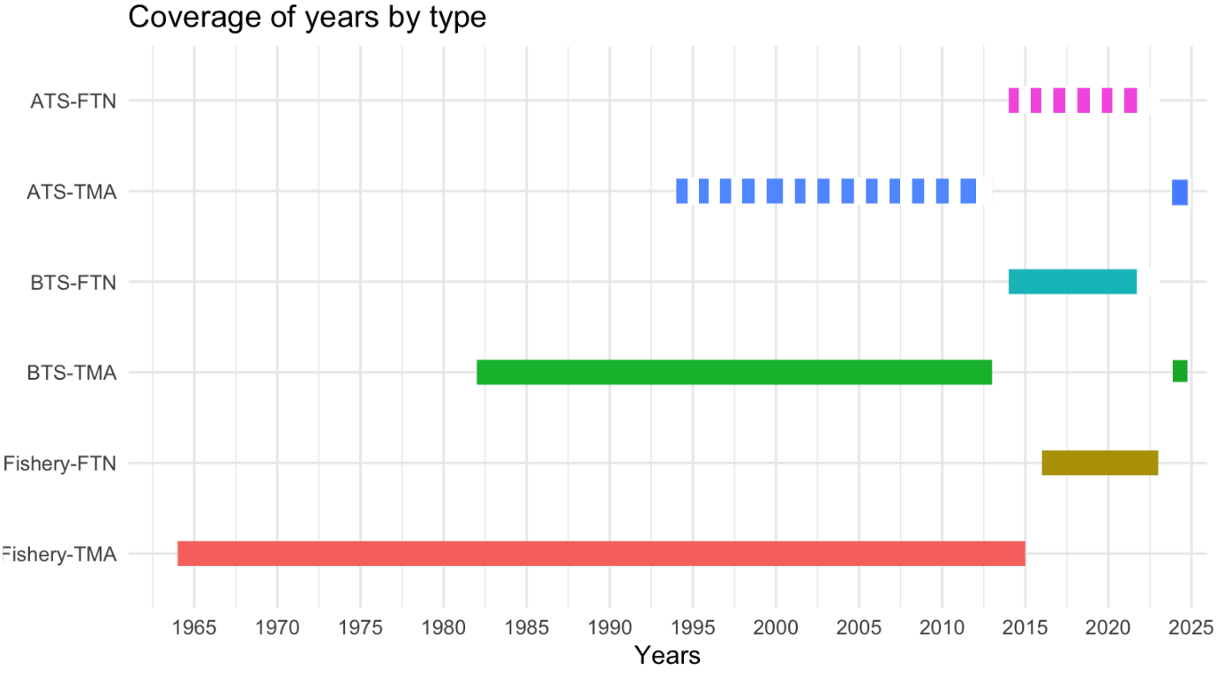
\includegraphics{doc/figs/DataExtent.png}

}

\caption{\label{fig-dataExtent}Data extent by age composition for the
models with FTNIRs age estimates. The data types are for the Fishery,
bottom trawl survey (BTS), and acoustic trawl survey (ATS) and the years
of coverage are shown in the x-axis.}

\end{figure}%

\section{Fit to models}\label{fit-to-models}

\begin{table}[ht]
\centering
\caption{Goodness-of-fit measures to primary data for different data and age-error applications.
RMSE=root-mean square log errors, NLL=negative log-likelihood, SDNR=standard deviation of normalized residuals,
Eff. N=effective sample size for composition data). See text for incremental model descriptions.} 
\label{tbl:modfits}
\begin{tabular}{lrrr}
  \hline
Component & Base & FT-NIR fleet-specific & FT-NIR fleets aggregated \\ 
  \hline
RMSE BTS & 0.15 & 0.15 & 0.15 \\ 
  RMSE ATS & 0.17 & 0.18 & 0.19 \\ 
  RMSE AVO & 0.22 & 0.24 & 0.24 \\ 
  RMSE CPUE & 0.10 & 0.10 & 0.10 \\ 
   \hline
SDNR BTS & 0.89 & 0.88 & 0.90 \\ 
  SDNR ATS & 0.93 & 1.07 & 1.13 \\ 
  SDNR AVO & 0.95 & 1.05 & 1.08 \\ 
   \hline
Eff. N Fishery & 357.67 & 380.56 & 335.24 \\ 
  Eff. N BTS & 159.43 & 152.12 & 147.18 \\ 
  Eff. N ATS & 233.17 & 227.21 & 214.61 \\ 
   \hline
Catch NLL & 2.96 & 3.01 & 4.25 \\ 
  BTS NLL & 23.91 & 23.43 & 24.41 \\ 
  ATS NLL & 7.75 & 10.08 & 11.39 \\ 
  AVO NLL & 8.24 & 10.06 & 10.53 \\ 
  Fish Age NLL & 416.81 & 613.35 & 558.82 \\ 
  BTS Age NLL & 286.12 & 314.10 & 330.37 \\ 
  ATS Age NLL & 42.55 & 45.97 & 46.97 \\ 
   \hline
NLL selectivity & 212.70 & 209.85 & 209.53 \\ 
  NLL Priors & 20.33 & 20.73 & 20.65 \\ 
   \hline
Data NLL & 807.12 & 1042.70 & 1007.77 \\ 
  Total NLL & 1110.90 & 1339.14 & 1305.93 \\ 
   \hline
\end{tabular}
\end{table}

\global\setlength{\Oldarrayrulewidth}{\arrayrulewidth}

\global\setlength{\Oldtabcolsep}{\tabcolsep}

\setlength{\tabcolsep}{2pt}

\renewcommand*{\arraystretch}{1.5}



\providecommand{\ascline}[3]{\noalign{\global\arrayrulewidth #1}\arrayrulecolor[HTML]{#2}\cline{#3}}

\begin{longtable*}[c]{|p{0.75in}|p{0.75in}|p{0.75in}|p{0.75in}}



\ascline{1.5pt}{666666}{1-4}

\multicolumn{1}{>{\raggedright}m{\dimexpr 0.75in+0\tabcolsep}}{\textcolor[HTML]{000000}{\fontsize{11}{11}\selectfont{\global\setmainfont{Arial}{Component}}}} & \multicolumn{1}{>{\raggedleft}m{\dimexpr 0.75in+0\tabcolsep}}{\textcolor[HTML]{000000}{\fontsize{11}{11}\selectfont{\global\setmainfont{Arial}{Base}}}} & \multicolumn{1}{>{\raggedleft}m{\dimexpr 0.75in+0\tabcolsep}}{\textcolor[HTML]{000000}{\fontsize{11}{11}\selectfont{\global\setmainfont{Arial}{FT-NIR\ fleets\ aggregated}}}} & \multicolumn{1}{>{\raggedleft}m{\dimexpr 0.75in+0\tabcolsep}}{\textcolor[HTML]{000000}{\fontsize{11}{11}\selectfont{\global\setmainfont{Arial}{FT-NIR\ fleet-specific}}}} \\

\ascline{1.5pt}{666666}{1-4}\endfirsthead 

\ascline{1.5pt}{666666}{1-4}

\multicolumn{1}{>{\raggedright}m{\dimexpr 0.75in+0\tabcolsep}}{\textcolor[HTML]{000000}{\fontsize{11}{11}\selectfont{\global\setmainfont{Arial}{Component}}}} & \multicolumn{1}{>{\raggedleft}m{\dimexpr 0.75in+0\tabcolsep}}{\textcolor[HTML]{000000}{\fontsize{11}{11}\selectfont{\global\setmainfont{Arial}{Base}}}} & \multicolumn{1}{>{\raggedleft}m{\dimexpr 0.75in+0\tabcolsep}}{\textcolor[HTML]{000000}{\fontsize{11}{11}\selectfont{\global\setmainfont{Arial}{FT-NIR\ fleets\ aggregated}}}} & \multicolumn{1}{>{\raggedleft}m{\dimexpr 0.75in+0\tabcolsep}}{\textcolor[HTML]{000000}{\fontsize{11}{11}\selectfont{\global\setmainfont{Arial}{FT-NIR\ fleet-specific}}}} \\

\ascline{1.5pt}{666666}{1-4}\endhead



\multicolumn{1}{>{\raggedright}m{\dimexpr 0.75in+0\tabcolsep}}{\textcolor[HTML]{000000}{\fontsize{11}{11}\selectfont{\global\setmainfont{Arial}{RMSE\ BTS}}}} & \multicolumn{1}{>{\raggedleft}m{\dimexpr 0.75in+0\tabcolsep}}{\textcolor[HTML]{000000}{\fontsize{11}{11}\selectfont{\global\setmainfont{Arial}{0.150}}}} & \multicolumn{1}{>{\raggedleft}m{\dimexpr 0.75in+0\tabcolsep}}{\textcolor[HTML]{000000}{\fontsize{11}{11}\selectfont{\global\setmainfont{Arial}{0.152}}}} & \multicolumn{1}{>{\raggedleft}m{\dimexpr 0.75in+0\tabcolsep}}{\textcolor[HTML]{000000}{\fontsize{11}{11}\selectfont{\global\setmainfont{Arial}{0.152}}}} \\





\multicolumn{1}{>{\raggedright}m{\dimexpr 0.75in+0\tabcolsep}}{\textcolor[HTML]{000000}{\fontsize{11}{11}\selectfont{\global\setmainfont{Arial}{RMSE\ ATS}}}} & \multicolumn{1}{>{\raggedleft}m{\dimexpr 0.75in+0\tabcolsep}}{\textcolor[HTML]{000000}{\fontsize{11}{11}\selectfont{\global\setmainfont{Arial}{0.167}}}} & \multicolumn{1}{>{\raggedleft}m{\dimexpr 0.75in+0\tabcolsep}}{\textcolor[HTML]{000000}{\fontsize{11}{11}\selectfont{\global\setmainfont{Arial}{0.192}}}} & \multicolumn{1}{>{\raggedleft}m{\dimexpr 0.75in+0\tabcolsep}}{\textcolor[HTML]{000000}{\fontsize{11}{11}\selectfont{\global\setmainfont{Arial}{0.184}}}} \\





\multicolumn{1}{>{\raggedright}m{\dimexpr 0.75in+0\tabcolsep}}{\textcolor[HTML]{000000}{\fontsize{11}{11}\selectfont{\global\setmainfont{Arial}{RMSE\ AVO}}}} & \multicolumn{1}{>{\raggedleft}m{\dimexpr 0.75in+0\tabcolsep}}{\textcolor[HTML]{000000}{\fontsize{11}{11}\selectfont{\global\setmainfont{Arial}{0.216}}}} & \multicolumn{1}{>{\raggedleft}m{\dimexpr 0.75in+0\tabcolsep}}{\textcolor[HTML]{000000}{\fontsize{11}{11}\selectfont{\global\setmainfont{Arial}{0.241}}}} & \multicolumn{1}{>{\raggedleft}m{\dimexpr 0.75in+0\tabcolsep}}{\textcolor[HTML]{000000}{\fontsize{11}{11}\selectfont{\global\setmainfont{Arial}{0.237}}}} \\





\multicolumn{1}{>{\raggedright}m{\dimexpr 0.75in+0\tabcolsep}}{\textcolor[HTML]{000000}{\fontsize{11}{11}\selectfont{\global\setmainfont{Arial}{RMSE\ CPUE}}}} & \multicolumn{1}{>{\raggedleft}m{\dimexpr 0.75in+0\tabcolsep}}{\textcolor[HTML]{000000}{\fontsize{11}{11}\selectfont{\global\setmainfont{Arial}{0.097}}}} & \multicolumn{1}{>{\raggedleft}m{\dimexpr 0.75in+0\tabcolsep}}{\textcolor[HTML]{000000}{\fontsize{11}{11}\selectfont{\global\setmainfont{Arial}{0.097}}}} & \multicolumn{1}{>{\raggedleft}m{\dimexpr 0.75in+0\tabcolsep}}{\textcolor[HTML]{000000}{\fontsize{11}{11}\selectfont{\global\setmainfont{Arial}{0.097}}}} \\





\multicolumn{1}{>{\raggedright}m{\dimexpr 0.75in+0\tabcolsep}}{\textcolor[HTML]{000000}{\fontsize{11}{11}\selectfont{\global\setmainfont{Arial}{SDNR\ BTS}}}} & \multicolumn{1}{>{\raggedleft}m{\dimexpr 0.75in+0\tabcolsep}}{\textcolor[HTML]{000000}{\fontsize{11}{11}\selectfont{\global\setmainfont{Arial}{0.890}}}} & \multicolumn{1}{>{\raggedleft}m{\dimexpr 0.75in+0\tabcolsep}}{\textcolor[HTML]{000000}{\fontsize{11}{11}\selectfont{\global\setmainfont{Arial}{0.900}}}} & \multicolumn{1}{>{\raggedleft}m{\dimexpr 0.75in+0\tabcolsep}}{\textcolor[HTML]{000000}{\fontsize{11}{11}\selectfont{\global\setmainfont{Arial}{0.880}}}} \\





\multicolumn{1}{>{\raggedright}m{\dimexpr 0.75in+0\tabcolsep}}{\textcolor[HTML]{000000}{\fontsize{11}{11}\selectfont{\global\setmainfont{Arial}{SDNR\ ATS}}}} & \multicolumn{1}{>{\raggedleft}m{\dimexpr 0.75in+0\tabcolsep}}{\textcolor[HTML]{000000}{\fontsize{11}{11}\selectfont{\global\setmainfont{Arial}{0.930}}}} & \multicolumn{1}{>{\raggedleft}m{\dimexpr 0.75in+0\tabcolsep}}{\textcolor[HTML]{000000}{\fontsize{11}{11}\selectfont{\global\setmainfont{Arial}{1.130}}}} & \multicolumn{1}{>{\raggedleft}m{\dimexpr 0.75in+0\tabcolsep}}{\textcolor[HTML]{000000}{\fontsize{11}{11}\selectfont{\global\setmainfont{Arial}{1.070}}}} \\





\multicolumn{1}{>{\raggedright}m{\dimexpr 0.75in+0\tabcolsep}}{\textcolor[HTML]{000000}{\fontsize{11}{11}\selectfont{\global\setmainfont{Arial}{SDNR\ AVO}}}} & \multicolumn{1}{>{\raggedleft}m{\dimexpr 0.75in+0\tabcolsep}}{\textcolor[HTML]{000000}{\fontsize{11}{11}\selectfont{\global\setmainfont{Arial}{0.950}}}} & \multicolumn{1}{>{\raggedleft}m{\dimexpr 0.75in+0\tabcolsep}}{\textcolor[HTML]{000000}{\fontsize{11}{11}\selectfont{\global\setmainfont{Arial}{1.080}}}} & \multicolumn{1}{>{\raggedleft}m{\dimexpr 0.75in+0\tabcolsep}}{\textcolor[HTML]{000000}{\fontsize{11}{11}\selectfont{\global\setmainfont{Arial}{1.050}}}} \\





\multicolumn{1}{>{\raggedright}m{\dimexpr 0.75in+0\tabcolsep}}{\textcolor[HTML]{000000}{\fontsize{11}{11}\selectfont{\global\setmainfont{Arial}{Eff.\ N\ Fishery}}}} & \multicolumn{1}{>{\raggedleft}m{\dimexpr 0.75in+0\tabcolsep}}{\textcolor[HTML]{000000}{\fontsize{11}{11}\selectfont{\global\setmainfont{Arial}{357.670}}}} & \multicolumn{1}{>{\raggedleft}m{\dimexpr 0.75in+0\tabcolsep}}{\textcolor[HTML]{000000}{\fontsize{11}{11}\selectfont{\global\setmainfont{Arial}{335.240}}}} & \multicolumn{1}{>{\raggedleft}m{\dimexpr 0.75in+0\tabcolsep}}{\textcolor[HTML]{000000}{\fontsize{11}{11}\selectfont{\global\setmainfont{Arial}{380.560}}}} \\





\multicolumn{1}{>{\raggedright}m{\dimexpr 0.75in+0\tabcolsep}}{\textcolor[HTML]{000000}{\fontsize{11}{11}\selectfont{\global\setmainfont{Arial}{Eff.\ N\ BTS}}}} & \multicolumn{1}{>{\raggedleft}m{\dimexpr 0.75in+0\tabcolsep}}{\textcolor[HTML]{000000}{\fontsize{11}{11}\selectfont{\global\setmainfont{Arial}{159.430}}}} & \multicolumn{1}{>{\raggedleft}m{\dimexpr 0.75in+0\tabcolsep}}{\textcolor[HTML]{000000}{\fontsize{11}{11}\selectfont{\global\setmainfont{Arial}{147.180}}}} & \multicolumn{1}{>{\raggedleft}m{\dimexpr 0.75in+0\tabcolsep}}{\textcolor[HTML]{000000}{\fontsize{11}{11}\selectfont{\global\setmainfont{Arial}{152.120}}}} \\





\multicolumn{1}{>{\raggedright}m{\dimexpr 0.75in+0\tabcolsep}}{\textcolor[HTML]{000000}{\fontsize{11}{11}\selectfont{\global\setmainfont{Arial}{Eff.\ N\ ATS}}}} & \multicolumn{1}{>{\raggedleft}m{\dimexpr 0.75in+0\tabcolsep}}{\textcolor[HTML]{000000}{\fontsize{11}{11}\selectfont{\global\setmainfont{Arial}{233.170}}}} & \multicolumn{1}{>{\raggedleft}m{\dimexpr 0.75in+0\tabcolsep}}{\textcolor[HTML]{000000}{\fontsize{11}{11}\selectfont{\global\setmainfont{Arial}{214.610}}}} & \multicolumn{1}{>{\raggedleft}m{\dimexpr 0.75in+0\tabcolsep}}{\textcolor[HTML]{000000}{\fontsize{11}{11}\selectfont{\global\setmainfont{Arial}{227.210}}}} \\





\multicolumn{1}{>{\raggedright}m{\dimexpr 0.75in+0\tabcolsep}}{\textcolor[HTML]{000000}{\fontsize{11}{11}\selectfont{\global\setmainfont{Arial}{Catch\ NLL}}}} & \multicolumn{1}{>{\raggedleft}m{\dimexpr 0.75in+0\tabcolsep}}{\textcolor[HTML]{000000}{\fontsize{11}{11}\selectfont{\global\setmainfont{Arial}{2.960}}}} & \multicolumn{1}{>{\raggedleft}m{\dimexpr 0.75in+0\tabcolsep}}{\textcolor[HTML]{000000}{\fontsize{11}{11}\selectfont{\global\setmainfont{Arial}{4.250}}}} & \multicolumn{1}{>{\raggedleft}m{\dimexpr 0.75in+0\tabcolsep}}{\textcolor[HTML]{000000}{\fontsize{11}{11}\selectfont{\global\setmainfont{Arial}{3.010}}}} \\





\multicolumn{1}{>{\raggedright}m{\dimexpr 0.75in+0\tabcolsep}}{\textcolor[HTML]{000000}{\fontsize{11}{11}\selectfont{\global\setmainfont{Arial}{BTS\ NLL}}}} & \multicolumn{1}{>{\raggedleft}m{\dimexpr 0.75in+0\tabcolsep}}{\textcolor[HTML]{000000}{\fontsize{11}{11}\selectfont{\global\setmainfont{Arial}{23.910}}}} & \multicolumn{1}{>{\raggedleft}m{\dimexpr 0.75in+0\tabcolsep}}{\textcolor[HTML]{000000}{\fontsize{11}{11}\selectfont{\global\setmainfont{Arial}{24.410}}}} & \multicolumn{1}{>{\raggedleft}m{\dimexpr 0.75in+0\tabcolsep}}{\textcolor[HTML]{000000}{\fontsize{11}{11}\selectfont{\global\setmainfont{Arial}{23.430}}}} \\





\multicolumn{1}{>{\raggedright}m{\dimexpr 0.75in+0\tabcolsep}}{\textcolor[HTML]{000000}{\fontsize{11}{11}\selectfont{\global\setmainfont{Arial}{ATS\ NLL}}}} & \multicolumn{1}{>{\raggedleft}m{\dimexpr 0.75in+0\tabcolsep}}{\textcolor[HTML]{000000}{\fontsize{11}{11}\selectfont{\global\setmainfont{Arial}{7.750}}}} & \multicolumn{1}{>{\raggedleft}m{\dimexpr 0.75in+0\tabcolsep}}{\textcolor[HTML]{000000}{\fontsize{11}{11}\selectfont{\global\setmainfont{Arial}{11.390}}}} & \multicolumn{1}{>{\raggedleft}m{\dimexpr 0.75in+0\tabcolsep}}{\textcolor[HTML]{000000}{\fontsize{11}{11}\selectfont{\global\setmainfont{Arial}{10.080}}}} \\





\multicolumn{1}{>{\raggedright}m{\dimexpr 0.75in+0\tabcolsep}}{\textcolor[HTML]{000000}{\fontsize{11}{11}\selectfont{\global\setmainfont{Arial}{AVO\ NLL}}}} & \multicolumn{1}{>{\raggedleft}m{\dimexpr 0.75in+0\tabcolsep}}{\textcolor[HTML]{000000}{\fontsize{11}{11}\selectfont{\global\setmainfont{Arial}{8.240}}}} & \multicolumn{1}{>{\raggedleft}m{\dimexpr 0.75in+0\tabcolsep}}{\textcolor[HTML]{000000}{\fontsize{11}{11}\selectfont{\global\setmainfont{Arial}{10.530}}}} & \multicolumn{1}{>{\raggedleft}m{\dimexpr 0.75in+0\tabcolsep}}{\textcolor[HTML]{000000}{\fontsize{11}{11}\selectfont{\global\setmainfont{Arial}{10.060}}}} \\





\multicolumn{1}{>{\raggedright}m{\dimexpr 0.75in+0\tabcolsep}}{\textcolor[HTML]{000000}{\fontsize{11}{11}\selectfont{\global\setmainfont{Arial}{Fish\ Age\ NLL}}}} & \multicolumn{1}{>{\raggedleft}m{\dimexpr 0.75in+0\tabcolsep}}{\textcolor[HTML]{000000}{\fontsize{11}{11}\selectfont{\global\setmainfont{Arial}{416.810}}}} & \multicolumn{1}{>{\raggedleft}m{\dimexpr 0.75in+0\tabcolsep}}{\textcolor[HTML]{000000}{\fontsize{11}{11}\selectfont{\global\setmainfont{Arial}{558.820}}}} & \multicolumn{1}{>{\raggedleft}m{\dimexpr 0.75in+0\tabcolsep}}{\textcolor[HTML]{000000}{\fontsize{11}{11}\selectfont{\global\setmainfont{Arial}{613.350}}}} \\





\multicolumn{1}{>{\raggedright}m{\dimexpr 0.75in+0\tabcolsep}}{\textcolor[HTML]{000000}{\fontsize{11}{11}\selectfont{\global\setmainfont{Arial}{BTS\ Age\ NLL}}}} & \multicolumn{1}{>{\raggedleft}m{\dimexpr 0.75in+0\tabcolsep}}{\textcolor[HTML]{000000}{\fontsize{11}{11}\selectfont{\global\setmainfont{Arial}{286.120}}}} & \multicolumn{1}{>{\raggedleft}m{\dimexpr 0.75in+0\tabcolsep}}{\textcolor[HTML]{000000}{\fontsize{11}{11}\selectfont{\global\setmainfont{Arial}{330.370}}}} & \multicolumn{1}{>{\raggedleft}m{\dimexpr 0.75in+0\tabcolsep}}{\textcolor[HTML]{000000}{\fontsize{11}{11}\selectfont{\global\setmainfont{Arial}{314.100}}}} \\





\multicolumn{1}{>{\raggedright}m{\dimexpr 0.75in+0\tabcolsep}}{\textcolor[HTML]{000000}{\fontsize{11}{11}\selectfont{\global\setmainfont{Arial}{ATS\ Age\ NLL}}}} & \multicolumn{1}{>{\raggedleft}m{\dimexpr 0.75in+0\tabcolsep}}{\textcolor[HTML]{000000}{\fontsize{11}{11}\selectfont{\global\setmainfont{Arial}{42.550}}}} & \multicolumn{1}{>{\raggedleft}m{\dimexpr 0.75in+0\tabcolsep}}{\textcolor[HTML]{000000}{\fontsize{11}{11}\selectfont{\global\setmainfont{Arial}{46.970}}}} & \multicolumn{1}{>{\raggedleft}m{\dimexpr 0.75in+0\tabcolsep}}{\textcolor[HTML]{000000}{\fontsize{11}{11}\selectfont{\global\setmainfont{Arial}{45.970}}}} \\





\multicolumn{1}{>{\raggedright}m{\dimexpr 0.75in+0\tabcolsep}}{\textcolor[HTML]{000000}{\fontsize{11}{11}\selectfont{\global\setmainfont{Arial}{NLL\ selectivity}}}} & \multicolumn{1}{>{\raggedleft}m{\dimexpr 0.75in+0\tabcolsep}}{\textcolor[HTML]{000000}{\fontsize{11}{11}\selectfont{\global\setmainfont{Arial}{212.700}}}} & \multicolumn{1}{>{\raggedleft}m{\dimexpr 0.75in+0\tabcolsep}}{\textcolor[HTML]{000000}{\fontsize{11}{11}\selectfont{\global\setmainfont{Arial}{209.530}}}} & \multicolumn{1}{>{\raggedleft}m{\dimexpr 0.75in+0\tabcolsep}}{\textcolor[HTML]{000000}{\fontsize{11}{11}\selectfont{\global\setmainfont{Arial}{209.850}}}} \\





\multicolumn{1}{>{\raggedright}m{\dimexpr 0.75in+0\tabcolsep}}{\textcolor[HTML]{000000}{\fontsize{11}{11}\selectfont{\global\setmainfont{Arial}{NLL\ Priors}}}} & \multicolumn{1}{>{\raggedleft}m{\dimexpr 0.75in+0\tabcolsep}}{\textcolor[HTML]{000000}{\fontsize{11}{11}\selectfont{\global\setmainfont{Arial}{20.330}}}} & \multicolumn{1}{>{\raggedleft}m{\dimexpr 0.75in+0\tabcolsep}}{\textcolor[HTML]{000000}{\fontsize{11}{11}\selectfont{\global\setmainfont{Arial}{20.650}}}} & \multicolumn{1}{>{\raggedleft}m{\dimexpr 0.75in+0\tabcolsep}}{\textcolor[HTML]{000000}{\fontsize{11}{11}\selectfont{\global\setmainfont{Arial}{20.730}}}} \\





\multicolumn{1}{>{\raggedright}m{\dimexpr 0.75in+0\tabcolsep}}{\textcolor[HTML]{000000}{\fontsize{11}{11}\selectfont{\global\setmainfont{Arial}{Data\ NLL}}}} & \multicolumn{1}{>{\raggedleft}m{\dimexpr 0.75in+0\tabcolsep}}{\textcolor[HTML]{000000}{\fontsize{11}{11}\selectfont{\global\setmainfont{Arial}{807.120}}}} & \multicolumn{1}{>{\raggedleft}m{\dimexpr 0.75in+0\tabcolsep}}{\textcolor[HTML]{000000}{\fontsize{11}{11}\selectfont{\global\setmainfont{Arial}{1,007.770}}}} & \multicolumn{1}{>{\raggedleft}m{\dimexpr 0.75in+0\tabcolsep}}{\textcolor[HTML]{000000}{\fontsize{11}{11}\selectfont{\global\setmainfont{Arial}{1,042.700}}}} \\





\multicolumn{1}{>{\raggedright}m{\dimexpr 0.75in+0\tabcolsep}}{\textcolor[HTML]{000000}{\fontsize{11}{11}\selectfont{\global\setmainfont{Arial}{Total\ NLL}}}} & \multicolumn{1}{>{\raggedleft}m{\dimexpr 0.75in+0\tabcolsep}}{\textcolor[HTML]{000000}{\fontsize{11}{11}\selectfont{\global\setmainfont{Arial}{1,110.900}}}} & \multicolumn{1}{>{\raggedleft}m{\dimexpr 0.75in+0\tabcolsep}}{\textcolor[HTML]{000000}{\fontsize{11}{11}\selectfont{\global\setmainfont{Arial}{1,305.930}}}} & \multicolumn{1}{>{\raggedleft}m{\dimexpr 0.75in+0\tabcolsep}}{\textcolor[HTML]{000000}{\fontsize{11}{11}\selectfont{\global\setmainfont{Arial}{1,339.140}}}} \\

\ascline{1.5pt}{666666}{1-4}



\end{longtable*}



\arrayrulecolor[HTML]{000000}

\global\setlength{\arrayrulewidth}{\Oldarrayrulewidth}

\global\setlength{\tabcolsep}{\Oldtabcolsep}

\renewcommand*{\arraystretch}{1}

\chapter{Leave-one-out sensitivity
analysis}\label{leave-one-out-sensitivity-analysis}

Here we present model runs that downweight one source of age composition
data at a time, as well as a run that downweights all survey biomass
indices.

\begin{figure}

\centering{

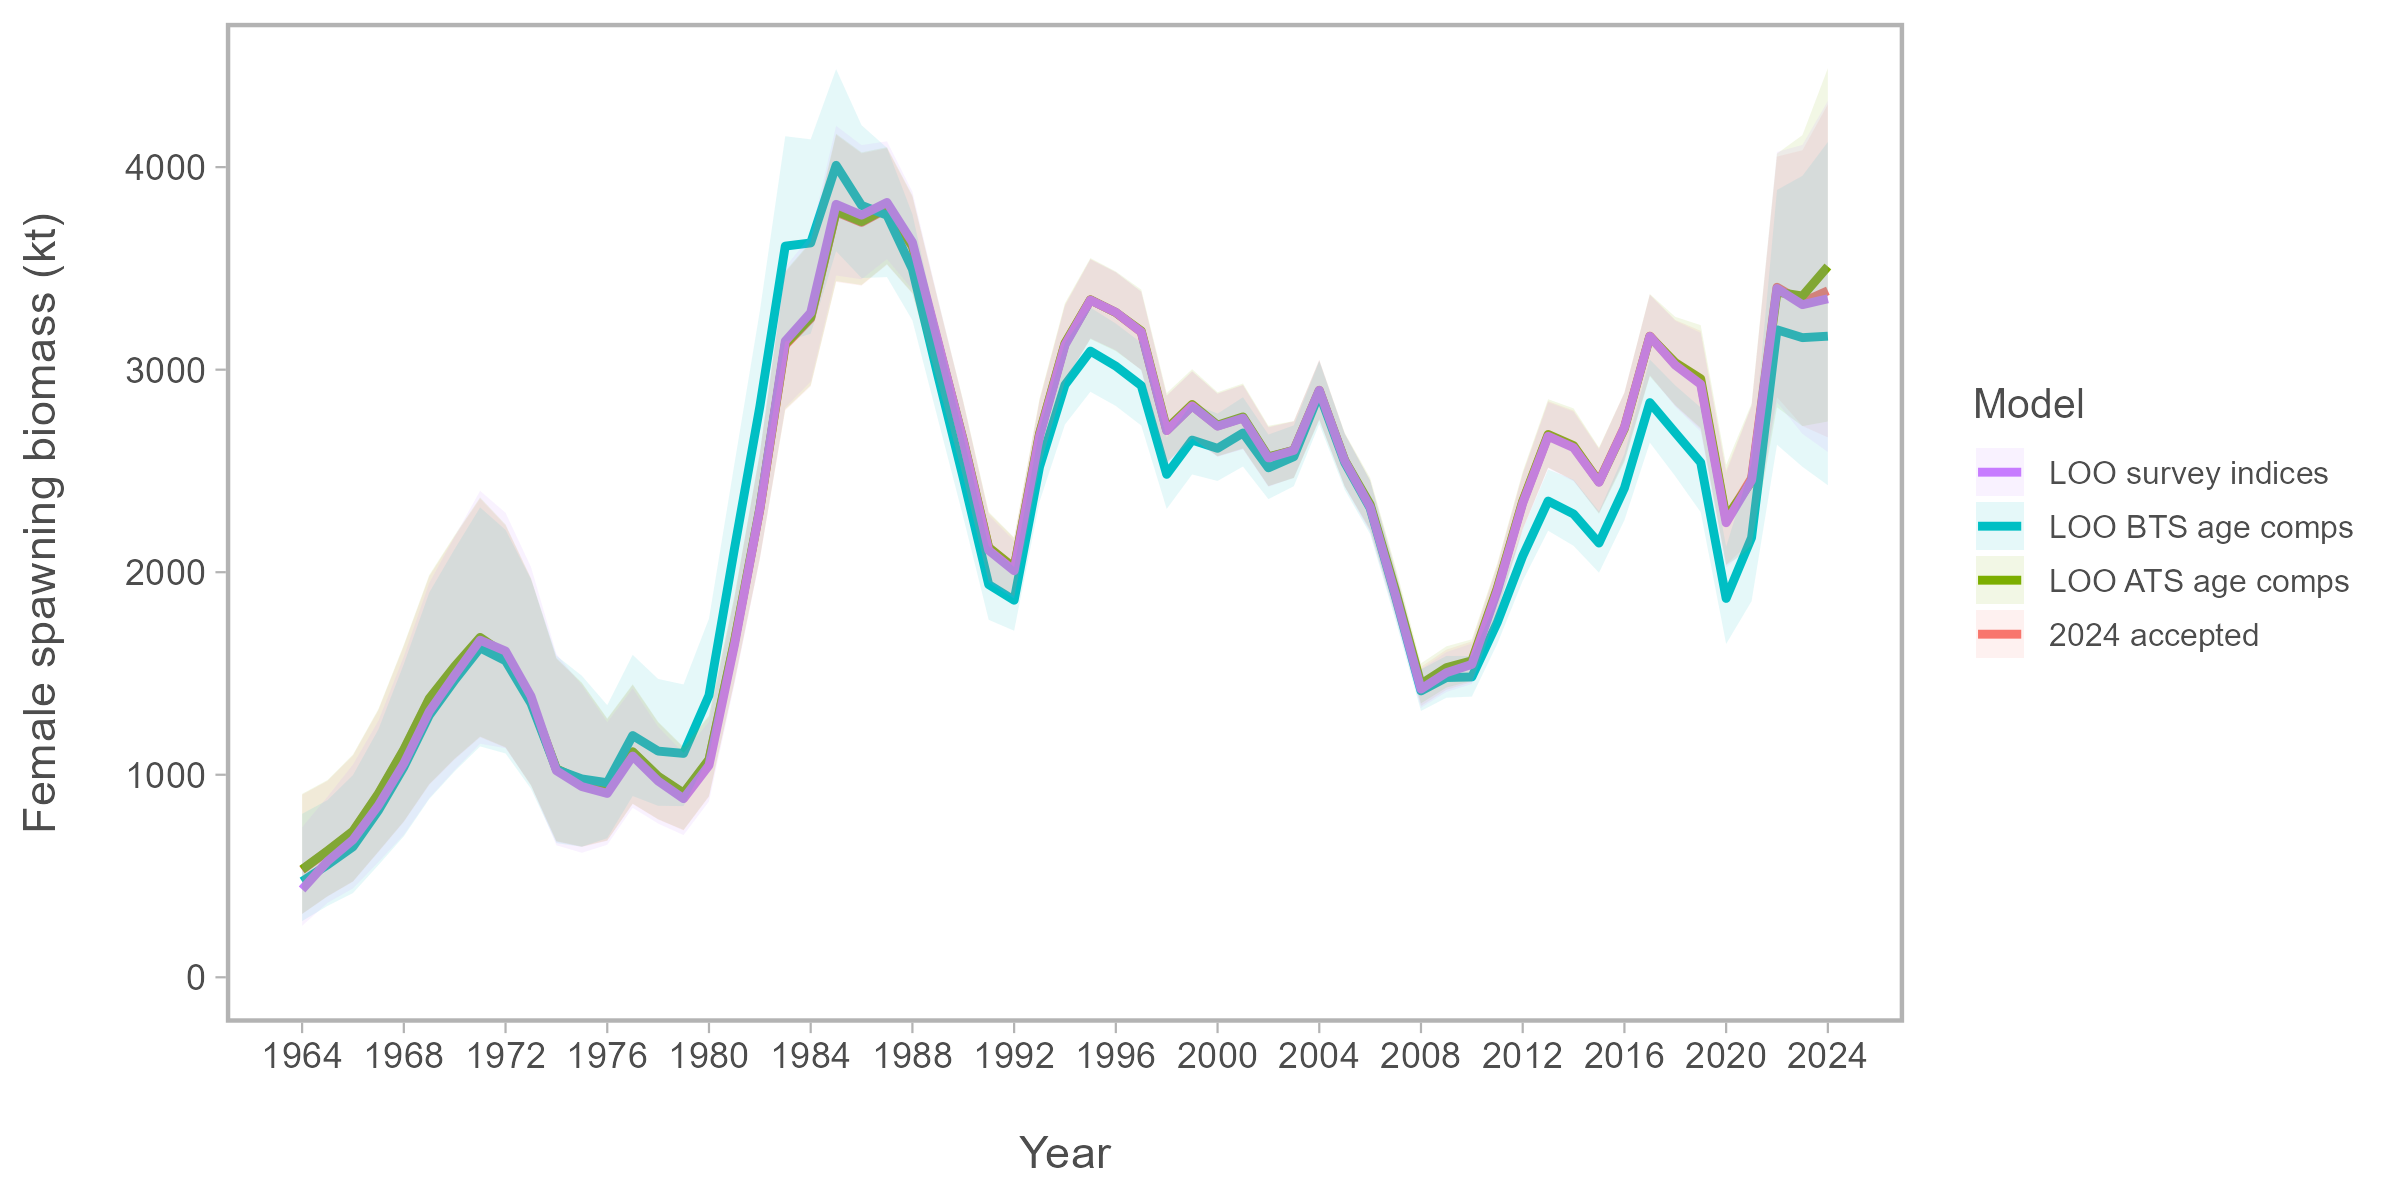
\includegraphics{doc/figs/loo_ssb.png}

}

\caption{\label{fig-loo}Model results comparing models that downweight
one data source at a time}

\end{figure}%

\chapter{Alternative assessment
software}\label{alternative-assessment-software}

\section{Stock-synthesis 3}\label{stock-synthesis-3}

Stock synthesis 3 (SS3) is a well establish framework and is common in
many diverse settings. (Methot and Wetzel (2013)) For EBS pollock, we
extended an initial framework based on the configurations used for
Pacific hake (Grandin et al. (2024)) since there are many similarities
in the type of data available. Namely, empirical weight-at-age, acoustic
survey data, and indices of 1-year olds (ref).

\section{WHAM}\label{wham}

The ``Woods Hole Assessment model'' (WHAM) is written in TMB and is a
fully state-space model (Stock and Miller (2021)).

\section{RTMB model}\label{rtmb-model}

Work at AFSC has developed a general model which has flexibility to
specify regions and a variety of options including random effects. While
this model is not yet fully developed, we present preliminary results
here. The model is written in TMB and is similar to the WHAM model. We
pursue this model to explore the potential for a more flexible model
that can be used for more explicit considerations of stocks linked to
different regions (e.g., the US and Russian portions of the EBS). Also,
this model to add sex-specificity and random effects (Cheng et al.
(2025)).

\section{CEATTLE model}\label{ceattle-model}

The CEATTLE model is a new model developed by the AFSC and is written in
TMB (Adams et al. (2022)). The model is an extension of the ADMB version
used for the three-species multi-species model (Jurado-Molina,
Livingston, and Ianelli (2005), Holsman et al. (2024)).

\chapter{Bottom-trawl survey spatial distribution
modeling}\label{bottom-trawl-survey-spatial-distribution-modeling}

Sophia's work here

\chapter*{References}\label{references}
\addcontentsline{toc}{chapter}{References}

\phantomsection\label{refs}
\begin{CSLReferences}{1}{0}
\bibitem[\citeproctext]{ref-adams2022}
Adams, Grant D., Kirstin K. Holsman, Steven J. Barbeaux, Martin W. Dorn,
James N. Ianelli, Ingrid Spies, Ian J. Stewart, and André E. Punt. 2022.
{``An Ensemble Approach to Understand Predation Mortality for Groundfish
in the Gulf of Alaska.''} \emph{Fisheries Research} 251: 106303.
https://doi.org/\url{https://doi.org/10.1016/j.fishres.2022.106303}.

\bibitem[\citeproctext]{ref-cheng2025}
Cheng, Matthew L. H., Daniel R. Goethel, Peter-John F. Hulson, Michael
J. Wilberg, Craig Marsh, and Curry J. Cunningham. 2025. {``Misspecifying
{Sex-Structured} {Dynamics} in {Stock} {Assessment} {Models}.''}
\emph{{Fish} and {Fisheries}}, February, 1--19.
\url{https://doi.org/10.1111/faf.12891}.

\bibitem[\citeproctext]{ref-hake2024}
Grandin, C. J., K. F. Johnson, A. M. Edwards, and A. M. Berger. 2024.
{``Status of the {Pacific} {Hake} (Whiting) Stock in {U.S.} And
{Canadian} Waters in 2024.''} Joint Technical Committee of the U.S.;
Canada Pacific Hake/Whiting Agreement, National Marine Fisheries
Service; Fisheries; Oceans Canada.

\bibitem[\citeproctext]{ref-helser2019}
Helser, Thomas E., Irina Benson, Jason Erickson, Jordan Healy, Craig
Kastelle, and Jonathan A. Short. 2019. {``A Transformative Approach to
Ageing Fish Otoliths Using Fourier Transform Near Infrared Spectroscopy:
A Case Study of Eastern Bering Sea Walleye Pollock ({\emph{Gadus
Chalcogrammus}}).''} \emph{Canadian Journal of Fisheries and Aquatic
Sciences} 76 (5): 780--89.
\url{https://doi.org/10.1139/cjfas-2018-0112}.

\bibitem[\citeproctext]{ref-holsman2024}
Holsman, K. K., J. Ianelli, K. Shotwell, S. Barbeaux, K. Aydin, G.
Adams, K. Kearney, A. Sulc, and S. Wassermann. 2024. {``Climate-Enhanced
Multispecies Stock Assessment for Walleye Pollock, {Pacific} Cod, and
Arrowtooth Flounder in the Eastern {Bering} {Sea}.''} Technical Report.
Anchorage, AK: North Pacific Fishery Management Council.
\url{https://www.npfmc.org/wp-content/PDFdocuments/SAFE/2024/EBSmultispp.pdf}.

\bibitem[\citeproctext]{ref-jurado2005}
Jurado-Molina, J., P. A. Livingston, and J. N. Ianelli. 2005.
{``Incorporating Predation Interactions to a Statistical Catch-at-Age
Model for a Predator-Prey System in the Eastern Bering Sea.''}
\emph{Canadian Journal of Fisheries and Aquatic Sciences} 62 (8):
1865--73.

\bibitem[\citeproctext]{ref-methot2013}
Methot, Richard D., and Chantell R. Wetzel. 2013. {``Stock Synthesis: A
Biological and Statistical Framework for Fish Stock Assessment and
Fishery Management.''} \emph{Fisheries Research} 142 (May): 86--99.
\url{https://doi.org/10.1016/j.fishres.2012.10.012}.

\bibitem[\citeproctext]{ref-punt2008}
Punt, A. E., D. C. Smith, K. KrusicGolub, and S. Robertson. 2008.
{``Quantifying Age-Reading Error for Use in Fisheries Stock Assessments,
with Application to Species in Australia's Southern and Eastern
Scalefish and Shark Fishery.''} \emph{Can. J. Fish. Aquat. Sci.} 65:
1991--2005.

\bibitem[\citeproctext]{ref-stock2021}
Stock, Brian C., and Timothy J. Miller. 2021. {``The {Woods Hole
Assessment Model} ({WHAM}): {A} General State-Space Assessment Framework
That Incorporates Time- and Age-Varying Processes via Random Effects and
Links to Environmental Covariates.''} \emph{Fisheries Research} 240
(August): 105967. \url{https://doi.org/10.1016/j.fishres.2021.105967}.

\end{CSLReferences}




\end{document}
